\documentclass[12pt,a4paper,twoside]{amsart}  % Package for mathematical article
\usepackage[T1]{fontenc}
\usepackage[utf8]{inputenc}

% Nice Font and some basic things
\usepackage{libertine}
\usepackage[libertine]{newtxmath}
\usepackage[nospace]{varioref}
\usepackage[ngerman,english]{babel}
\usepackage{mathrsfs}  % For using mathsrc and not overwriting mathcal
\usepackage[top=3cm,bottom=2.5cm,left=3cm,right=2.5cm]{geometry}
\usepackage{float}
\usepackage{graphicx}

\usepackage{parskip} % Use spaces between paragraphs instead of parindent
\setlength{\parskip}{0.3\baselineskip plus 2pt} 
\raggedbottom % Do not stretch content on a page instead leave an empty space in the bottom 
\sloppy  % This can help with linebreaks but is possibly bad for overfull hboxes
\usepackage{etoolbox} % to do the following
\AtBeginEnvironment{proof}{\vspace*{-2\parskip}} % Avoid big space at begin of proof

% Nice Referencing
\usepackage{xurl} % For nice url formatting
\usepackage{hyperref} % Se hypersetup below
\urlstyle{same}
\usepackage[noabbrev]{cleveref}

% Math packages
\usepackage{mathtools}
\usepackage{amsthm}
\usepackage{derivative} % For partial derivatives with \pdv{function}{variables}
\usepackage{dsfont} % For the indicator function \mathds{1}

% New math commands that are formated for math mode
\DeclareMathOperator{\img}{Im}
\DeclareMathOperator{\sign}{sign}
\DeclareMathOperator{\id}{Id}
\DeclareMathOperator{\vol}{vol}
\DeclareMathOperator{\hodgestar}{\ast}
\DeclareMathOperator{\Hom}{Hom}

% Other commands
\newcommand{\interior}[1]{{\kern0pt#1}^{\mathrm{o}}}
\newcommand{\into}{\hookrightarrow}
\newcommand{\onto}{\twoheadrightarrow}
\newcommand{\opartial}{{\overline{\partial}}}


\usepackage{enumitem} % Control the format of \enumerate \itemize and \description
\renewcommand\labelitemi{--} % This doesn't belong to package enumitem but can be used to customize itemize

% Definitions for amsthm
\theoremstyle{plain}
\newtheorem{thm}{Theorem}[subsection]
\newtheorem*{thm*}{Theorem}
\newtheorem{lm}[thm]{Lemma}
\newtheorem{prop}[thm]{Proposition}
\newtheorem{cor}[thm]{Corollary}
\newtheorem{fact}[thm]{Fact}
\newtheorem{q}[thm]{Question}
\theoremstyle{definition}
\newtheorem{defn}[thm]{Definition}
\newtheorem{nota}[thm]{Notation}
\newtheorem{exmp}[thm]{Example}
\newtheorem{xca}[thm]{Exercise}
\newtheorem*{set}{Setting}
\theoremstyle{remark}
\newtheorem{rem}[thm]{Remark}
\Crefname{thm}{Theorem}{Theorems}
\Crefname{lm}{Lemma}{Lemmas}
\Crefname{prop}{Proposition}{Propositions}
\Crefname{cor}{Corollary}{Corollaries}
\Crefname{fact}{Fact}{Facts}
\Crefname{q}{Question}{Questions}
\Crefname{defn}{Definition}{Definitions}
\Crefname{nota}{Notation}{Notations}
\Crefname{exmp}{Example}{Examples}
\Crefname{xca}{Exercise}{Exercises}
\Crefname{rem}{Remark}{Remarks}

\Crefname{enumi}{Property}{Properties} % For a nice referenceing of lists (label needs to be after \item)
\newcommand{\creflmpart}[2]{%
	\nameCref{#1}~\hyperref[#2]{\labelcref*{#1}~(\ref*{#2})}%
}

\Crefname{equation}{}{} % Set referencing style of equation to empy

\usepackage{tikz-cd} % For plots and drawings
\usetikzlibrary{decorations.markings}

\usepackage{float} % positioning figures and tables
\renewcommand\thepart{\rm \Roman{part}} % Nicer indentation of lists
\setdescription{labelindent=1 em, leftmargin=2 em}
\setitemize[1]{labelindent=1 em, leftmargin=2 em}
\setenumerate[1]{labelindent=0cm, leftmargin=*, widest=iiii}

% Bibliography
\usepackage[
backend=biber,
style=alphabetic,
maxnames=10,
maxalphanames=10,
url=true]{biblatex}
\addbibresource{./bibliography.bib}

% TODO functionality:
\usepackage{xcolor}
\newcommand\TODO[1]{\textcolor{red}{#1}}
% If all todo should be hidden at once just uncomment this line
% \renewcommand\TODO[1]{}
\newcommand\CITATION[1]{\textcolor{green}{#1}}


% Begin of document
\title{Minimum Lap Time Optimization}
\author{Álvaro Galisteo Bermúdez, Daniel Rath, Anastasiia Kliushnik}
\date{\today}

\setcounter{tocdepth}{2}  % Show sections and subsections in table of contents
\numberwithin{equation}{section} % Equations should have their own counter and should be numbered within a section to get (sectionnumber.equation)


\makeatletter %----------------------------------------------

% Setup hyperref
\hypersetup{
	pdfauthor={\authors},
	pdftitle={\@title},
	colorlinks,
	linkcolor=[rgb]{0.2,0.2,0.6},
	citecolor=[rgb]{0.2,0.6,0.2},
	urlcolor=[rgb]{0.6,0.2,0.2}}
\makeatother
%----------------------------------------------

% commands for temporarily enabling and disabling toc entires
\let\oldaddcontentsline\addcontentsline
\newcommand{\stoptocentries}{\renewcommand{\addcontentsline}[3]{}}
\newcommand{\starttocentries}{\let\addcontentsline\oldaddcontentsline}

% Begin of document -----------------------------------------
\begin{document}
	\newgeometry{
		includeall,
		bindingoffset=0cm,
		margin=2cm,
		marginparsep=0cm,
		marginparwidth=0cm,
		top=0cm
	}
	\begin{abstract}
    This report studies minimum-lap-time trajectory optimization for a vehicle on a closed racing track. The problem is formulated using a kinematic bicycle model in Frenet coordinates and transcribed by direct multiple shooting with fourth-order Runge–Kutta integration. The resulting nonlinear optimization problem is implemented in CasADi and solved with IPOPT under track, vehicle, and control constraints.\\
	The optimized trajectory exploits the available track width and adapts the vehicle speed to the local track curvature. The formulation is further extended to include static obstacles represented by elliptical safety regions. The resulting trajectory successfully avoids all obstacles while causing only a small increase in the optimal lap time.\\
	This report documents the final project for the lecture \emph{Numerical Optimization}, offered in the summer term 2026 within the master’s program \emph{Mathematics in Data and Technology} at the University of Freiburg.
	\end{abstract}
	
	
    \maketitle
	\tableofcontents
	\newpage
    \restoregeometry
	\pagenumbering{arabic}
	\section{The problem setup}
\TODO{Here we need to explain:\\
\begin{enumerate}
    \item What we want to do / optimize? 
    \item Wich data we know ? 
    \item What assumpions we use ? 
\end{enumerate}
}
	\section{Vehicle model}
The vehicle model must capture the main relationship between steering, longitudinal motion, and the resulting trajectory while remaining sufficiently simple for the numerical optimization problem. Since this project focuses on the minimum-lap-time optimization problem rather than on detailed vehicle dynamics, we use a kinematic bicycle model.

The kinematic bicycle model describes the vehicle motion using only a few states and control inputs. It is simple enough for numerical optimization while still capturing the main effects of steering and acceleration. More detailed effects, such as tire slip, load transfer, suspension motion, and transient tire forces, are neglected.
\subsection{The bicycle model}\;\\
The commonly used kinematic bicycle model is a simplification of the dynamics of a car. It represents the two wheels of each axle by a single equivalent wheel, resulting in one front wheel and one rear wheel. Only the front wheel is used for steering, and tire slip is neglected.

The model is described by the position of the car in global coordinates $(x,y)$, the velocity $v$, the heading $\psi$, and the steering angle $\delta$. The dynamics of the model are given by
\begin{align*}
    \dot{x} &= v \cos(\psi) \\
    \dot{y} &= v \sin(\psi) \\
    \dot{\psi} &= \frac{v}{L} \tan(\delta) \\
    \dot{v} &= a
\end{align*}
The parameter $L$ denotes the wheelbase of the car, i.e. the distance between the front and rear wheel, and the acceleration of the car respectively. For more details on this model, see \cite{Rajamani2012}.

However, for driving around a given track it is inconvenient to use global coordinates because it is more complicate to formulate the constraints. Additionally, we only need the position on the track and do not care for the absolute position in global coordinates.

Therefore, we want to formulate the model using track coordinates. The centerline distance traveled will be given as $s$ and $e_y$ denotes the distance from the centerline, $e_\psi$ denotes the angle between the cars heading and the tangent of the centerline and $v$ still denotes the velocity of the vehicle.

The position of the vehicle can be expressed relative to the track centerline as
\begin{align*}
    \mathbf{p}(t)
    =
    \mathbf{p}_c(s(t))
    +
    e_y(t)\mathbf{N}(s(t)),
\end{align*}
where $\mathbf{p}_c(s)$ denotes the centerline position and
$\mathbf{N}(s)$ is its unit normal vector.

Differentiating with respect to time gives
\begin{align*}
    \dot{\mathbf{p}}
    &=
    \frac{d\mathbf{p}_c}{ds}\dot{s}
    +
    \dot{e}_y\mathbf{N}
    +
    e_y\frac{d\mathbf{N}}{ds}\dot{s}.
\end{align*}
Using
\begin{align*}
    \frac{d\mathbf{p}_c}{ds}=\mathbf{T},
    \qquad
    \frac{d\mathbf{N}}{ds}=-\kappa(s)\mathbf{T},
\end{align*}
where $\mathbf{T}(s)$ is the unit tangent vector, we obtain
\begin{align*}
    \dot{\mathbf{p}}
    =
    \left(1-\kappa(s)e_y\right)\dot{s}\,\mathbf{T}
    +
    \dot{e}_y\,\mathbf{N}.
\end{align*}

The vehicle velocity can also be decomposed into components tangent and
normal to the centerline:
\begin{align*}
    \dot{\mathbf{p}}
    =
    v\cos(e_\psi)\mathbf{T}
    +
    v\sin(e_\psi)\mathbf{N}.
\end{align*}

Equating the tangential and normal components gives
\begin{align*}
    \left(1-\kappa(s)e_y\right)\dot{s}
    &=
    v\cos(e_\psi), \\
    \dot{e}_y
    &=
    v\sin(e_\psi).
\end{align*}
Therefore,
\begin{align*}
    \dot{s}
    =
    \frac{v\cos(e_\psi)}
    {1-\kappa(s)e_y}.
\end{align*}
This relation is commonly used in Frenet-coordinate formulations of vehicle
dynamics \cite{Reiter2023Frenet}.

The heading error is defined as
\begin{align*}
    e_\psi = \psi-\psi_c(s),
\end{align*}
where $\psi_c(s)$ denotes the heading of the track centerline.

Differentiating with respect to time and applying the chain rule yields
\begin{align*}
    \dot e_\psi
    =
    \dot\psi
    -
    \frac{d\psi_c}{ds}\dot s.
\end{align*}

The cars own heading with respect to the tangent of the centerline changes because of steering and the heading of the track changes because of the curvature of the track.

Since the derivative of the centerline heading with respect to the arc length is equal to the local track curvature,
\begin{align*}
    \frac{d\psi_c}{ds}=\kappa(s),
\end{align*}
the heading-error dynamics become

\begin{align*}
    \dot e_\psi = \frac{v}{L} \tan(\delta) - \kappa(s)\dot s.
\end{align*}

This results in the following vehicle model expressed in Frenet coordinates.
The state vector is defined as
\begin{align*}
    z(t)
    =
    \begin{bmatrix}
        s(t)\\
        e_y(t)\\
        e_\psi(t)\\
        v(t)
    \end{bmatrix},
\end{align*}
where \(s(t)\) denotes the progress along the track centerline,
\(e_y(t)\) the lateral offset from the centerline,
\(e_\psi(t)\) the heading error, and \(v(t)\) the vehicle velocity.

The control vector is given by
\begin{align*}
    u(t)
    =
    \begin{bmatrix}
        a(t)\\
        \delta(t)
    \end{bmatrix},
\end{align*}
where \(a(t)\) is the longitudinal acceleration and \(\delta(t)\) is the
steering angle.

The state dynamics can then be written compactly as
\begin{align*}
    \dot z(t)
    =
    f\bigl(z(t),u(t)\bigr)
    =
    \begin{bmatrix}
        \dfrac{v(t)\cos(e_\psi(t))}
        {1-\kappa(s(t))e_y(t)}
        \\[3ex]
        v(t)\sin(e_\psi(t))
        \\[1.5ex]
        \dfrac{v(t)}{L}\tan(\delta(t))
        -
        \kappa(s(t))
        \dfrac{v(t)\cos(e_\psi(t))}
        {1-\kappa(s(t))e_y(t)}
        \\[1.5ex]
        a(t)
    \end{bmatrix}.
\end{align*}

The kinematic bicycle model neglects tire slip, load transfer,
suspension dynamics and transient tire forces.
Consequently, it is not intended to accurately describe the vehicle behaviour
at the limits of adhesion.

Nevertheless, it captures the main relationship between steering,
longitudinal acceleration and the resulting vehicle trajectory while keeping
the optimization problem sufficiently simple.
	\section{Optimization Problem}
\subsection{Formulation of the optimization problem}\;\\
Using the vehicle model introduced in the previous section, the minimum-lap-time problem can be formulated as a continuous-time optimal control problem. The decision variables are the state trajectory $z(\cdot)$, the control trajectory $u(\cdot)$, and the final time $T$.

The control vector
\begin{align*}
    u(t) = \begin{bmatrix} a(t) \\ \delta(t) \end{bmatrix}
\end{align*}
contains the longitudinal acceleration and the steering angle.

The objective is to minimize the total time required to complete the track. 
The resulting optimal control problem is
\begin{align}
    \underset{z(\cdot),\,u(\cdot),\,T}{\operatorname{minimize}}
    \quad & T
    \label{eq:objective}
    \\[0.5em]
    \text{subject to}
    \quad
    & \dot{z}(t)
    =
    f\bigl(z(t),u(t)\bigr),
    && t\in[0,T],
    \label{eq:dynamics}
    \\[0.3em]
    & -\frac{w\bigl(s(t)\bigr)-b}{2}
    \leq e_y(t)
    \leq
    \frac{w\bigl(s(t)\bigr)-b}{2},
    && t\in[0,T],
    \label{eq:track_constraint}
    \\[0.3em]
    & -a_{\min}
    \leq a(t)
    \leq a_{\max},
    && t\in[0,T],
    \label{eq:acceleration_constraint}
    \\[0.3em]
    & -\delta_{\max}
    \leq \delta(t)
    \leq \delta_{\max},
    && t\in[0,T],
    \label{eq:steering_constraint}
    \\[0.3em]
    & 0
    \leq v(t)
    \leq v_{\max},
    && t\in[0,T],
    \label{eq:velocity_constraint}
    \\[0.3em]
    & -a_{y,\max}
    \leq
    \frac{v(t)^2}{L}\tan\bigl(\delta(t)\bigr)
    \leq
    a_{y,\max},
    && t\in[0,T],
    \label{eq:lateral_acceleration_constraint}
    \\[0.3em]
    & 1-\kappa\bigl(s(t)\bigr)e_y(t)>0,
    && t\in[0,T],
    \label{eq:frenet_validity_constraint}
    \\[0.3em]
    & s(0)=0,
    \qquad
    s(T)=S,
    \label{eq:position_boundary_conditions}
    \\[0.3em]
    & v(0)=0,
    \qquad
    e_y(0)=0,
    \qquad
    e_\psi(0)=0,
    \label{eq:initial_conditions}
    \\[0.3em]
    & T>0.
    \label{eq:time_constraint}
\end{align}

The parameters appearing in the optimal control problem are defined as follows:
\begin{description}
    \item[\(w(s)\)] track width at centerline position \(s\),
    \item[\(b\)] vehicle width,
    \item[\(L\)] vehicle wheelbase,
    \item[\(a_{\min}>0\)] magnitude of the maximum permissible deceleration,
    \item[\(a_{\max}>0\)] maximum permissible acceleration,
    \item[\(\delta_{\max}\)] maximum absolute steering angle,
    \item[\(v_{\max}\)] maximum permissible velocity,
    \item[\(a_{y,\max}\)] maximum permissible lateral acceleration,
    \item[\(S\)] total centerline length of the track.
\end{description}

The objective function~\eqref{eq:objective} minimizes the final time $T$.
The dynamic constraint~\eqref{eq:dynamics} ensures that the state trajectory
is consistent with the kinematic bicycle model.

The track constraint~\eqref{eq:track_constraint} restricts the center of the
vehicle to the usable track width. The vehicle width $b$ is subtracted from
the track width so that the complete vehicle, rather than only its reference
point, remains inside the track boundaries.

The acceleration, steering, and velocity constraints
\eqref{eq:acceleration_constraint}--\eqref{eq:velocity_constraint} represent
the longitudinal and kinematic limitations of the vehicle. The lateral
acceleration constraint~\eqref{eq:lateral_acceleration_constraint} limits the
cornering acceleration generated by the steering input.

The boundary conditions require the vehicle to start at the beginning of the
track and reach the total centerline distance $S$. In the present formulation,
the vehicle starts from rest at the centerline with zero heading error.


\subsection{Extension: Static obstacle avoidance.}\;\\
So far, the optimization problem only considers the track boundaries and vehicle limitations. In practical racing scenarios, however, additional objects may occupy parts of the track. To account for such situations, the formulation can be extended by introducing static obstacles represented in Frenet coordinates.

The positions of the obstacles are assumed to be known in advance and are specified in Frenet coordinates. For each obstacle $i=1,\ldots,N_{\mathrm{obs}}$, the centerline position is denoted by $s_i$ and the lateral offset by $e_{y,i}$. Furthermore, each obstacle is assigned a length $l_i$ and a width $w_i$.

To account for the finite dimensions of both the obstacle and the vehicle, together with an additional safety margin, each obstacle is surrounded by an elliptical safety region. The corresponding semi-axes in the longitudinal and lateral directions are defined as
\begin{align*}
    & r_{s,i}=\frac{l_i}{2}+\frac{L}{2}+d_{\mathrm{safe}},
    \\
    & r_{e_y,i}=\frac{w_i}{2}+\frac{b}{2}+d_{\mathrm{safe}},
\end{align*}
where $L$ denotes the vehicle wheelbase, $b$ its width, and $d_{\mathrm{safe}}$ the prescribed safety margin.

For every obstacle, the vehicle is required to remain outside the corresponding safety region. This requirement is enforced by introducing the nonlinear constraint
\begin{align}
\left(\frac{s-s_i}{r_{s,i}}\right)^2
+
\left(\frac{e_y-e_{y,i}}{r_{e_y,i}}\right)^2
\ge 1,
\qquad i=1,\ldots,N_{\mathrm{obs}}.
\end{align}

Since the optimization problem is solved on a discrete time grid, obstacle avoidance constraints are additionally evaluated at the midpoint of every integration interval. This improves collision detection between consecutive discretization nodes while avoiding the computational expense of using a much finer discretization.

This extension illustrates how additional practical constraints can be integrated into the optimal control formulation without modifying the underlying vehicle model.
	\section{Numerical solution}
\TODO{We need to cover here: 
\begin{enumerate}
    \item Discretization
    \item Multiple-shooting
    \item CasAdi
    \item IPOPT (or other solver use)
\end{enumerate}
}
	\section{Results}

The optimization problem was solved using \(N=200\) shooting intervals. IPOPT converged successfully after 357 iterations, requiring approximately \(8.0~\mathrm{s}\) of computation time. The solver returned the status \texttt{Solve\_Succeeded}. The optimal lap time obtained was

\begin{equation}
    T^*=61.665~\mathrm{s}.
\end{equation}

The main numerical results are summarized in Table~\ref{tab:optimization_results}.

\begin{table}[htbp]
    \centering
    \caption{Main optimization results for \(N=200\).}
    \label{tab:optimization_results}
    \begin{tabular}{lc}
        \hline
        Quantity & Result \\
        \hline
        Optimal lap time & \(61.665~\mathrm{s}\) \\
        Mean velocity & \(11.864~\mathrm{m/s}\) \\
        Maximum velocity & \(12.500~\mathrm{m/s}\) \\
        Lateral-offset range & \([-2.870,\ 2.870]~\mathrm{m}\) \\
        Acceleration range & \([-6.000,\ 3.000]~\mathrm{m/s^2}\) \\
        Steering-angle range & \([-0.600,\ 0.126]~\mathrm{rad}\) \\
        Lateral-acceleration range & \([-8.000,\ 8.000]~\mathrm{m/s^2}\) \\
        Minimum Frenet denominator & \(0.6827\) \\
        IPOPT iterations & \(357\) \\
        Computation time & \(7.996~\mathrm{s}\) \\
        Solver status & \texttt{Solve\_Succeeded} \\
        \hline
    \end{tabular}
\end{table}

Figure~\ref{fig:trajectory} shows the reconstructed track together with the optimized trajectory. Rather than following the centerline, the vehicle moves across the available track width to obtain smoother cornering lines and reduce the lap time.

\begin{figure}[htbp]
    \centering
    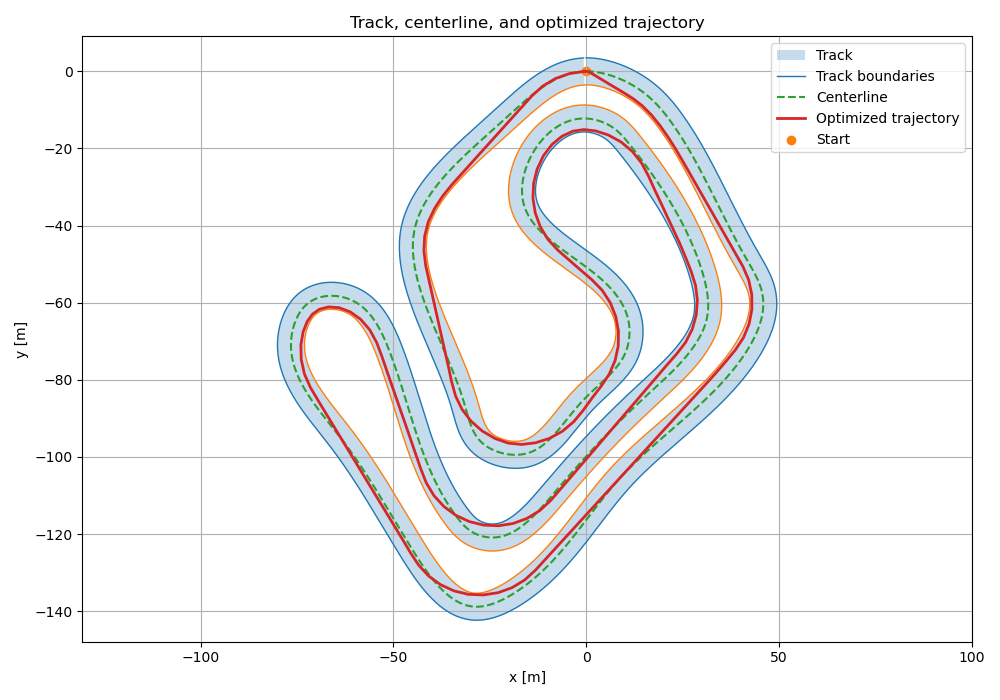
\includegraphics[width=0.70\linewidth]{images/track_optimzed_traj.png}
    \caption{Reconstructed track geometry, centerline and optimized trajectory.}
    \label{fig:trajectory}
\end{figure}

The corresponding lateral displacement is shown in Figure~\ref{fig:lateral}. The optimizer makes use of almost the entire admissible width, reaching the limits of \(\pm2.87~\mathrm{m}\) in several corners. This behaviour is consistent with an optimal racing line, where the vehicle moves towards the outside before entering a corner and approaches the inside near the apex.

\begin{figure}[htbp]
    \centering
    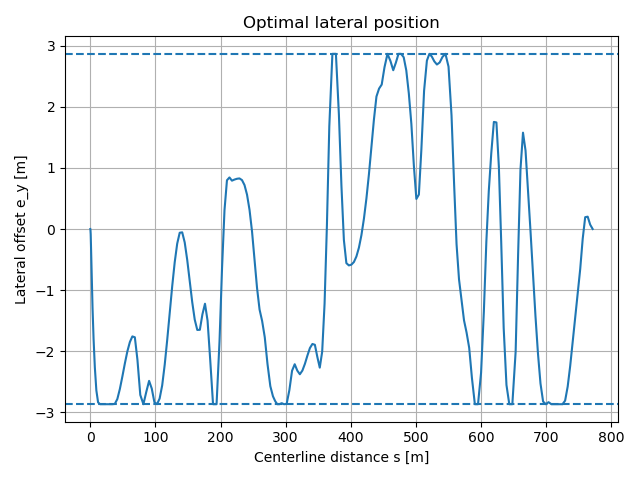
\includegraphics[width=0.70\linewidth]{images/opt_lat_pos.png}
    \caption{Optimized lateral displacement with admissible track limits.}
    \label{fig:lateral}
\end{figure}

The optimal velocity profile is presented in Figure~\ref{fig:velocity}. The kart rapidly accelerates to the maximum allowed speed of \(12.5~\mathrm{m/s}\) and remains close to this value over most of the circuit. Speed reductions only occur in the sections with the highest curvature, where the lateral-acceleration constraint becomes active.

\begin{figure}[htbp]
    \centering
    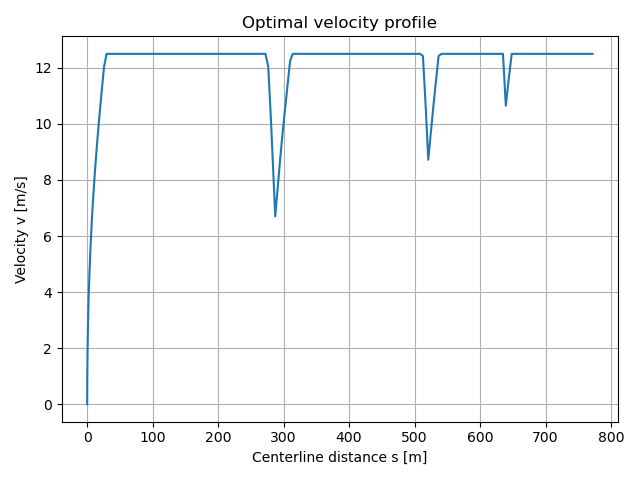
\includegraphics[width=0.70\linewidth]{images/vel_profile.png}
    \caption{Optimal velocity profile along the track centerline.}
    \label{fig:velocity}
\end{figure}

The longitudinal acceleration varies between \(-6.0\) and \(3.0~\mathrm{m/s^2}\), while the lateral acceleration reaches the imposed limits of \(\pm8.0~\mathrm{m/s^2}\). This indicates that both the longitudinal and lateral capabilities of the vehicle are fully exploited during the lap. The steering angle remains within the prescribed bounds, ranging from \(-0.600\) to \(0.126~\mathrm{rad}\).

Finally, the minimum value of the Frenet-coordinate denominator is

\[
\min(1-\kappa e_y)=0.6827,
\]

which remains well above zero throughout the optimization. Therefore, the computed trajectory stays within the valid region of the Frenet-coordinate formulation.
	\thispagestyle{empty}
	\printbibliography
\end{document}